\documentclass[11pt]{article}
\usepackage{geometry,marginnote} % Pour passer au format A4
\geometry{hmargin=1cm, vmargin=1cm} % 

% Page et encodage
\usepackage[T1]{fontenc} % Use 8-bit encoding that has 256 glyphs
\usepackage[english,french]{babel} % Français et anglais
\usepackage[utf8]{inputenc} 

\usepackage{lmodern,numprint}
\setlength\parindent{0pt}

% Graphiques
\usepackage{graphicx,float,grffile,units}
\usepackage{tikz,pst-eucl,pst-plot,pstricks,pst-node,pstricks-add,pst-fun,pgfplots} 

% Maths et divers
\usepackage{amsmath,amsfonts,amssymb,amsthm,verbatim}
\usepackage{multicol,enumitem,url,eurosym,gensymb,tabularx}

\DeclareUnicodeCharacter{20AC}{\euro}



% Sections
\usepackage{sectsty} % Allows customizing section commands
\allsectionsfont{\centering \normalfont\scshape}

% Tête et pied de page
\usepackage{fancyhdr} \pagestyle{fancyplain} \fancyhead{} \fancyfoot{}

\renewcommand{\headrulewidth}{0pt} % Remove header underlines
\renewcommand{\footrulewidth}{0pt} % Remove footer underlines

\newcommand{\horrule}[1]{\rule{\linewidth}{#1}} % Create horizontal rule command with 1 argument of height

\newcommand{\Pointilles}[1][3]{%
  \multido{}{#1}{\makebox[\linewidth]{\dotfill}\\[\parskip]
}}

\newtheorem{Definition}{Définition}

\usepackage{siunitx}
\sisetup{
    detect-all,
    output-decimal-marker={,},
    group-minimum-digits = 3,
    group-separator={~},
    number-unit-separator={~},
    inter-unit-product={~}
}

\setlength{\columnseprule}{1pt}

\begin{document}

\section*{3 - Les nombres relatifs : Introduction}

\begin{Definition}{Nombres relatifs}\\
  L'ensemble des nombres positifs et négatifs s'appelle les nombres relatifs.
\end{Definition}

\subsection*{1 - Des exemples}

Les nombres négatifs ne se trouve pas de partout. Ils sont néanmoins assez courants.

\textit{Remarque : négatif vient du latin \textbf{negare} qui signifie nier.}

\begin{multicols}{3}
\begin{enumerate}
  \item[1.] La température.
  \begin{figure}[H]
    \centering
    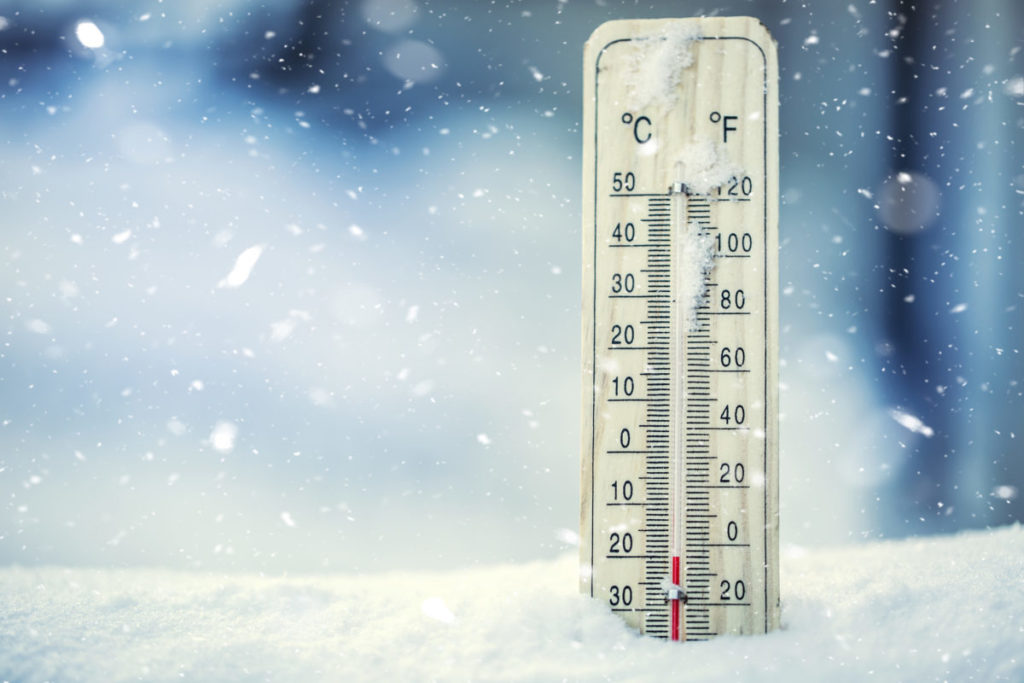
\includegraphics[width=0.8\linewidth]{5x3-nombres-relatifs-1-intro/c-temp.png}
  \end{figure}
  \item[2.] L'altitude sous la mer.
  \begin{figure}[H]
    \centering
    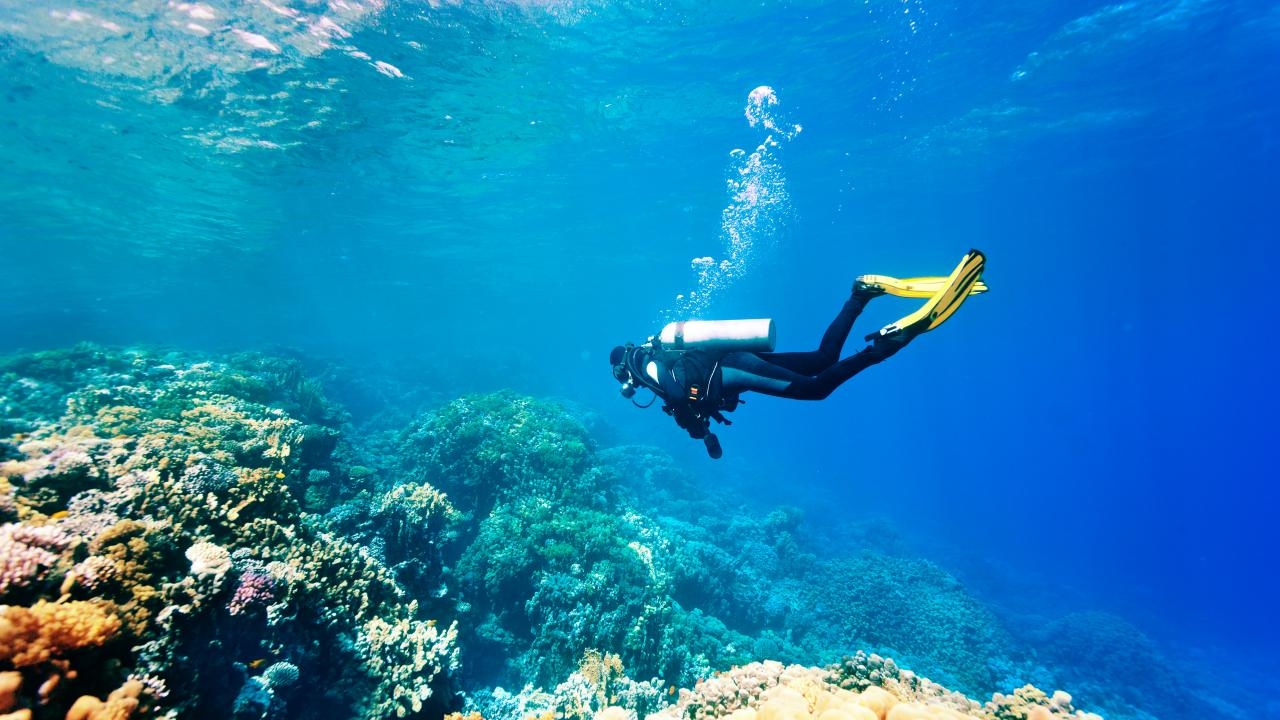
\includegraphics[width=0.8\linewidth]{5x3-nombres-relatifs-1-intro/c-plongee.png}
  \end{figure} \columnbreak

  \item[3.] Les étages d'ascenseurs.
  \begin{figure}[H]
    \centering
    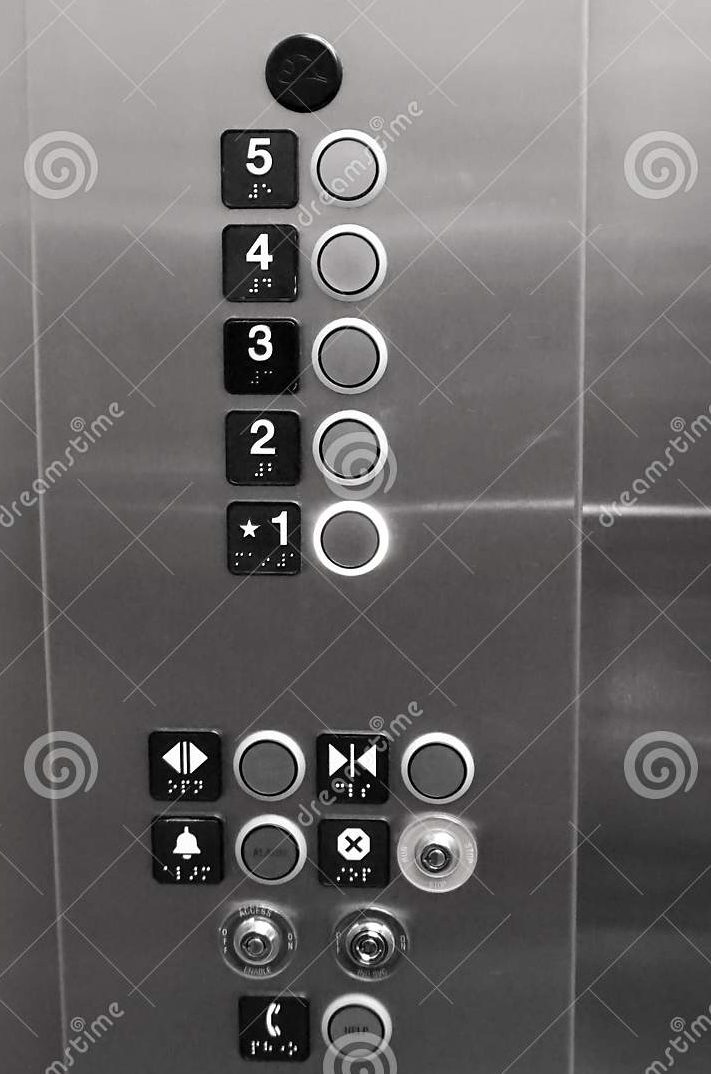
\includegraphics[width=0.8\linewidth]{5x3-nombres-relatifs-1-intro/c-ascenseur.png}
  \end{figure} \columnbreak

  \item[4.] Les dettes d'argents. 
  \begin{figure}[H]
    \centering
    
\includegraphics[width=0.8\linewidth]{5x3-nombres-relatifs-1-intro/c-argent.png}
  \end{figure}
  \item[5.] En électricité. 
  \begin{figure}[H]
    \centering
    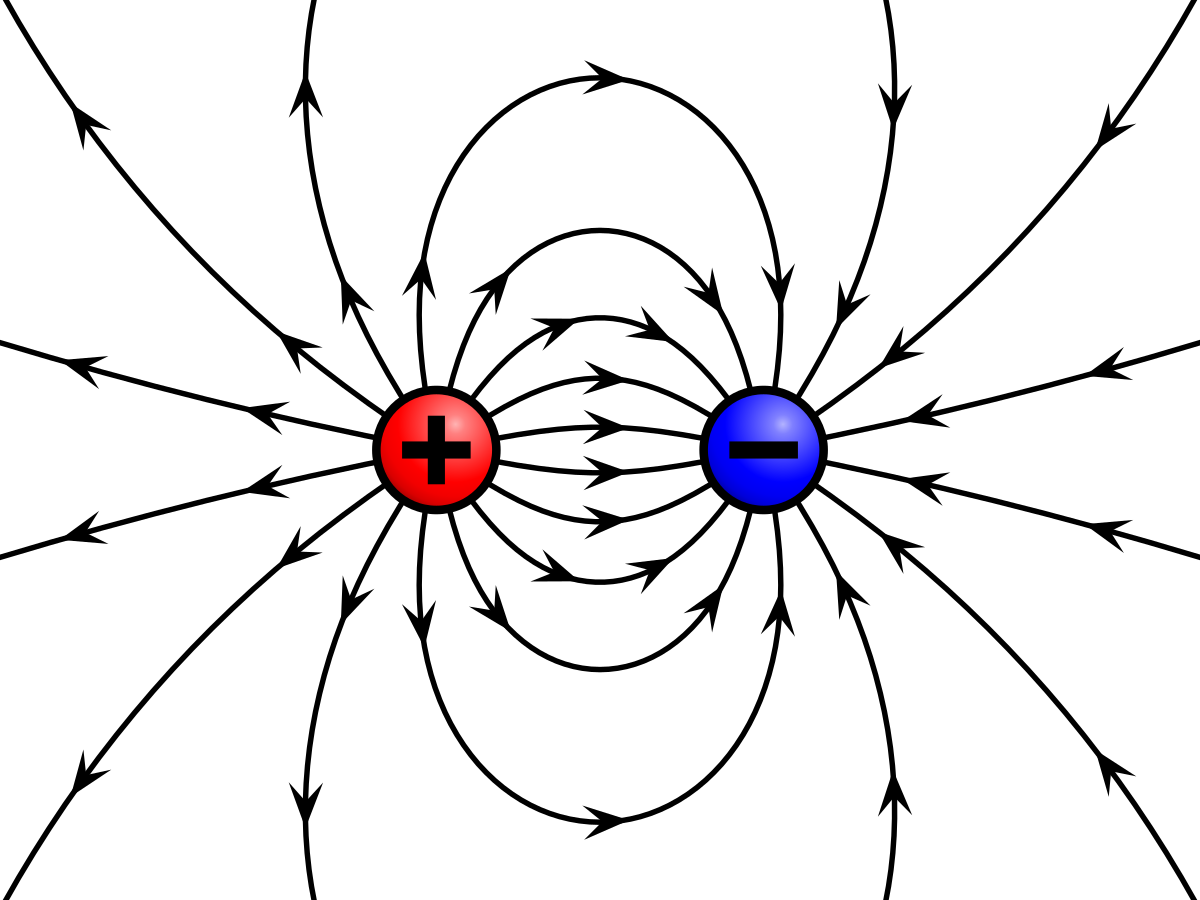
\includegraphics[width=0.8\linewidth]{5x3-nombres-relatifs-1-intro/c-elec.png}
  \end{figure} 
\end{enumerate}
\end{multicols}

\subsection*{2 - Les nombres négatifs}

On a besoin d'une nouvelle notation pour écrire les nombres négatifs. On utilise le symbole $-$. Sur les calculatrices TI, on utilise une nouvelle touche.\\


\begin{Definition}{Un nombre négatif}\\
  Un nombre négatif est un nombre plus petit que 0. \\
  $-0 - 5 = -5$
\end{Definition}


\subsection*{3 - Les opposés}

\begin{Definition}{Opposé}\\
  Deux nombres sont opposés si leur somme est nulle. \newline
  $-5$ est l'opposé de $5$ car :

  \begin{itemize}[label={$\bullet$}]
    \item $-5 + 5 = 0$
    \item $5 + -5 = 0$ 
  \end{itemize} 
\end{Definition}

\textbf{Remarque : } Additionner ne veut pas toujours dire ajouter. 
\end{document}
